The CMS tracker is the innermost layer of CMS, and is composed of silicon pixel and strip trackers. The main purpose of the tracker is to detect tracks left by electrically charged particles. These tracks are used to measure particle momentum, corresponding to the track's radius. Additionally, the tracker is used to identify the sign of the particle's charge, and is crucial for identifying the vertex of hard interactions from LHC collisions. The tracker is the most sensitive of the CMS sub-detectors, and is subject to the brunt of radiation produced by LHC collisions.  

\subsubsection{Pixel tracker} \label{sec:PIXEL}

The innermost layer of the CMS detector, and first layer of the CMS tracker, is the pixel tracker. This pixel tracker is composed of silicon sensors, of which there were initially about 65 million individual pixel readout channels in 2016. After the first full year of Run 2 data taking in 2016, the pixel detector was upgraded to the Phase-I pixel detector \cite{PhaseI_Pixel} in order to maintain performance following the upgrade of the LHC during the first Long Shutdown (LS1) from 2013-14, from which an instantaneous luminosity larger than the original pixel detector design was produced. The Phase-I pixel detector was installed during the 2016 Year End Technical Stop (YETS), which lasted from December 2016 to April 2017. After its installation, the Phase-I pixel detector, now containing about 124 million individual channels, was used during the 2017 and 2018 data-taking periods of Run 2.

The pixel tracker is composed of the Barrel (BPIX) and Forward (FPIX) pixel detectors, which result in a combined pseudorapidity region for particle detection of $|\eta| < 2.5$. A layout of the Phase-I pixel detector, and a comparison to the original design, is shown in Figure \ref{fig:Pixel_Tracker}. 

% \begin{figure}[H]
%     \centering % trim=left botm right top
%     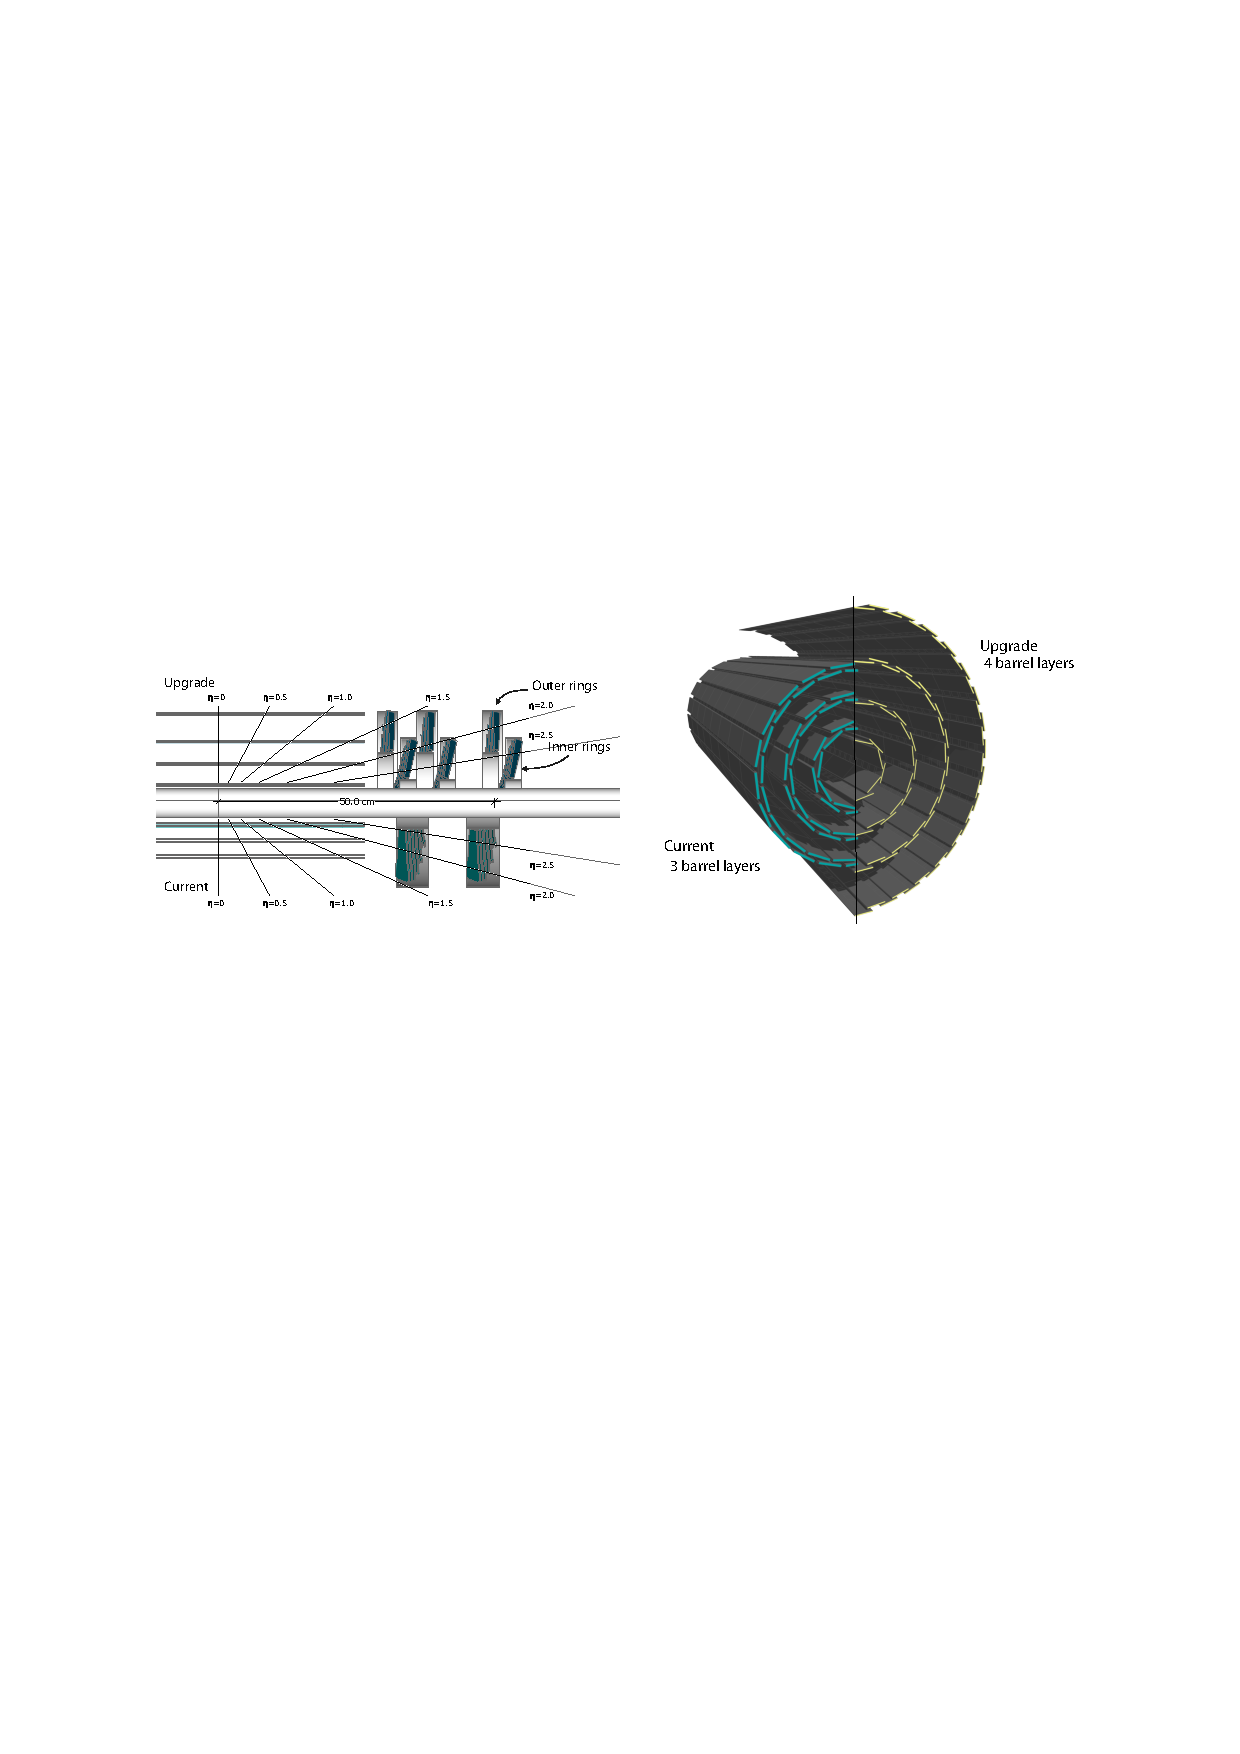
\includegraphics[clip, trim=0cm 0cm 0cm 6cm , width=\textwidth]{Images/CMS/Tracker/Tracker_Phase_Compare.pdf}
%     \caption{The Phase-I CMS pixel detector (upper), compared to its original design (lower).}
%     \label{fig:Pixel_Tracker}
% \end{figure}

\begin{figure}[H]
    \centering % trim=left botm right top
    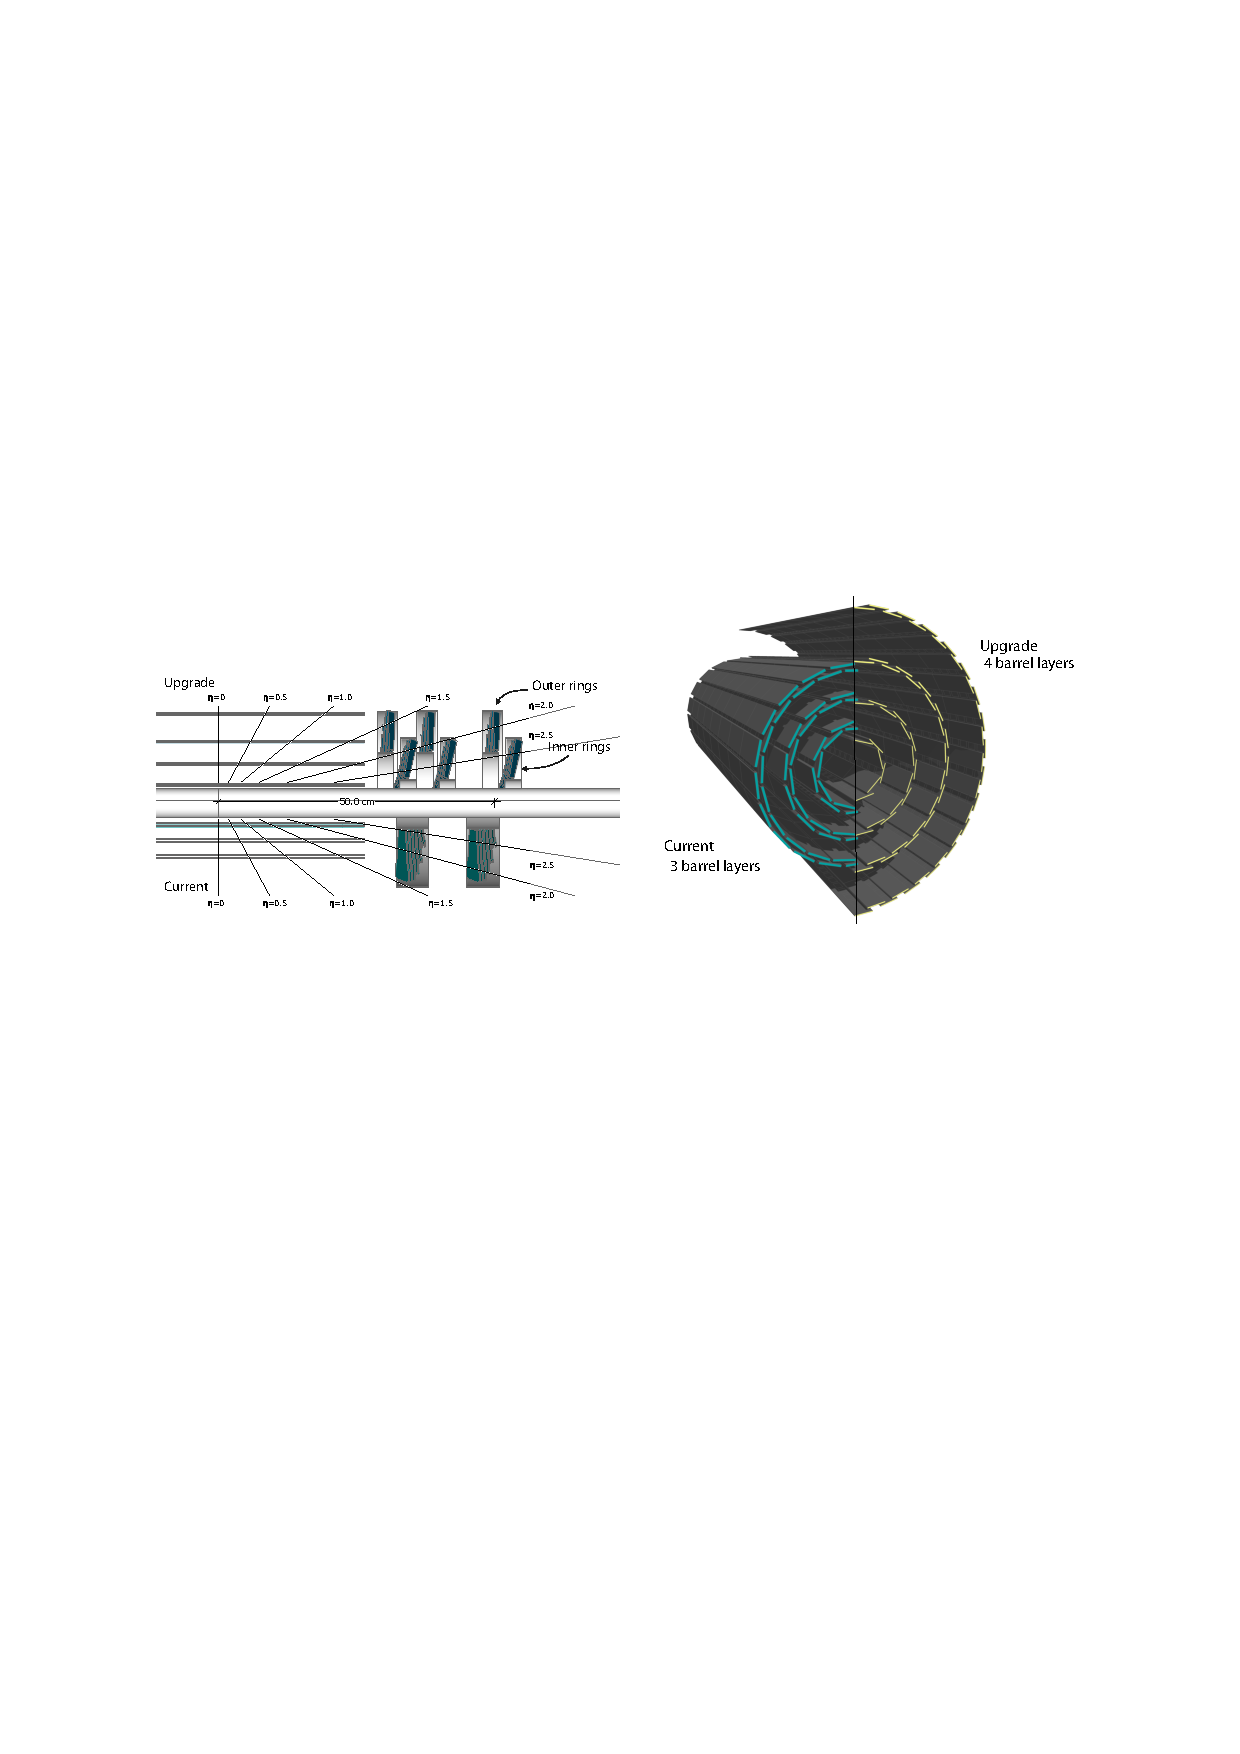
\includegraphics[width=\textwidth]{Images/CMS/Tracker/Tracker_Phase_Compare.pdf}
    \caption{The Phase-I CMS pixel detector (``Upgrade"), compared to its original design (``Current").}
    \label{fig:Pixel_Tracker}
\end{figure}

It can be seen that the main additions to the original CMS pixel detector are the addition of a layer in BPIX, and the addition of several disks in FPIX. Half of the BPIX system during production is shown in Figure \ref{fig:BPIX_Half}. In this image, the four half-circles concentric to the center of the image correspond to the four layers, L1-4. 

\begin{figure}[H]
    \centering
    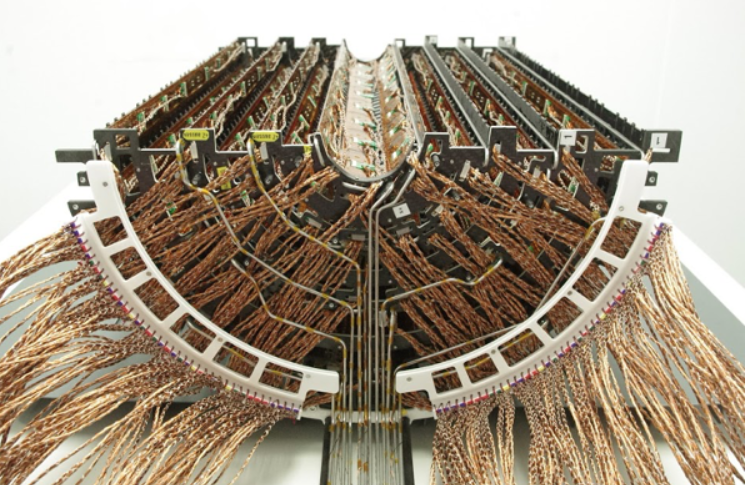
\includegraphics[width=0.7\textwidth]{Images/CMS/Tracker/BPIX.png}
    \caption{Half of the Phase-I BPIX.}
    \label{fig:BPIX_Half}
\end{figure}

The Phase-I pixel detector was able to deliver its expected performance, as shown in Figure \ref{fig:PIX_HitEfficiency}. 

\begin{figure}[H]
    \centering
    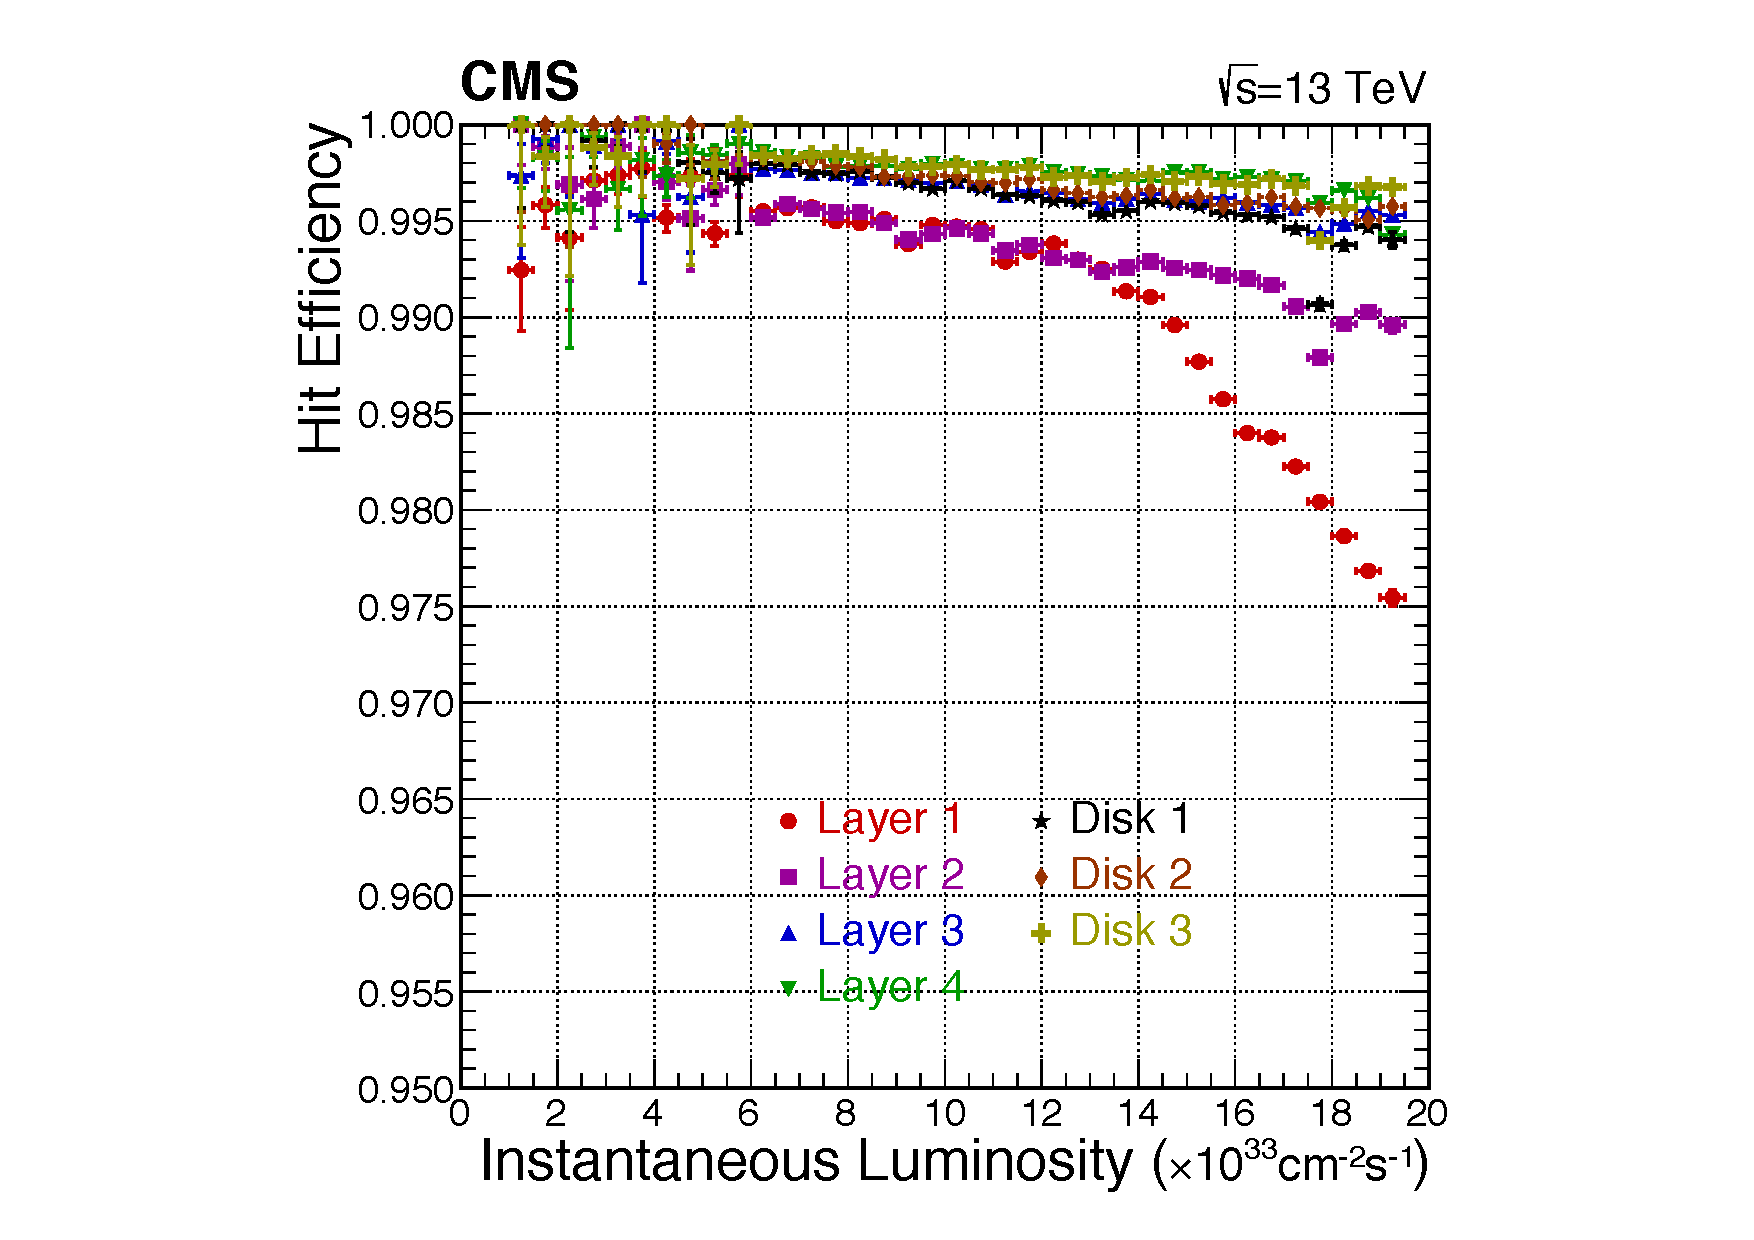
\includegraphics[width=\textwidth]{Images/CMS/Tracker/Pixel_HitEfficiency.pdf}
    \caption{Pixel hit efficiency during 2018.}
    \label{fig:PIX_HitEfficiency}
\end{figure}

The hit efficiency is shown as a function of different instantaneous luminosities during the 2018 data-taking year of Run 2, where higher values correspond to a higher number of simultaneous interactions, and therefore harsher data-taking conditions. Hit efficiency is defined as the probability that a cluster of pixel hits corresponds to an extrapolated track. Layers 1-3 of BPIX, and the entire FPIX were able to maintain hit efficiencies around 99\% even for large instantaneous luminosity values of 2*$ 10^{34}$cm$^{-2}$s$^{-1}$. Additionally, the L1 hit efficiency, which suffers the most from the harsh data-taking conditions at it is closest to the interaction region, begins to drop around 1.4*$10^{34}$cm$^{-2}$s$^{-1}$ down to about 97.5\% at 2cm$10^{34}^{-2}$s$^{-1}$. However, this performance is greater than what would have been expected from the original pixel tracker which ran during 2016. 

This is an example of a detector upgrade which was unforeseen but deemed necessary to implement, in response to the data-taking conditions presented to CMS based on collisions delivered by the LHC.

\subsubsection{Strip tracker}

% https://pos.sissa.it/309/013/pdf
% https://twiki.cern.ch/twiki/bin/view/CMSPublic/DPGResultsTRK

The second layer of the CMS detector, and outer portion of the CMS tracker, is the strip tracker. A view of one quarter of the Phase I strip tracker used during Run 2 can be seen in Figure \ref{fig:Strip_Tracker}. 

\begin{figure}[H]
    \centering
    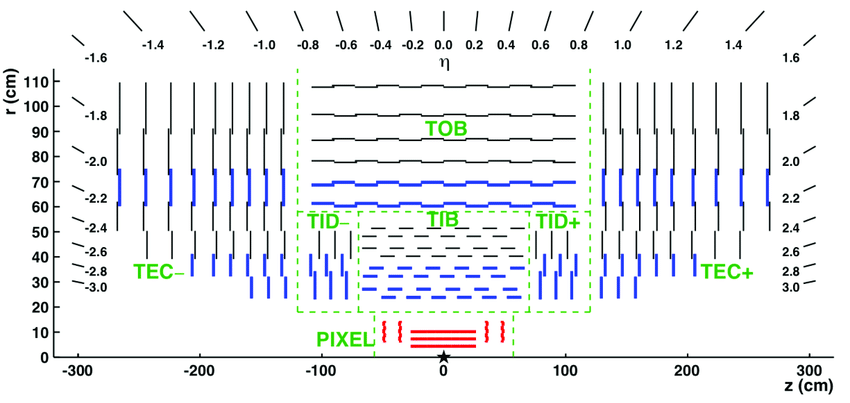
\includegraphics[width=0.7\textwidth]{Images/CMS/Tracker/upper-Schematic-view-of-the-CMS-tracker-detector-1-and-lower-closeup-view-of-the.png}    
    \caption{A view of half of the CMS strip detector in the r-z plane of CMS.}
    \label{fig:Strip_Tracker}
\end{figure}

The CMS strip tracker is composed of 15,148 silicon sensors which are spread over several partitions to cover different regions around the collision point: The Tracker Outer Barrel (TOB), Tracker Inner Barrel (TIB), Tracker Inner Disks (TID) with a plus and minus side, and Tracker Endcaps (TEC) which have modules on the plus and minus side. As shown in the diagram, the strip tracker surrounds the pixel tracker described in Section \ref{sec:PIXEL}. 

The strip tracker performs the same task as the pixel tracker, namely recording hits from electromagnetically charged particles in order to track their movement - a vital task for measuring particle $p_{T}$, identifying interaction vertices, and identifying jets from quark/gluon hadronization. The pixel and strip measurements are combined in order to obtain more accurate track measurements.  

During Run 2, the strip tracker maintained an excellent signal over noise ratio, and held a very stable percentage of problematic channels during Run 2, shown in Figure \ref{fig:Run2_StripTracker}.

\begin{figure}[H]% 
    \setcounter{subfigure}{0} % reset subcaption counter to 0 (a) 
    \centering
    \subfloat[2017 Signal over noise of TIB ]{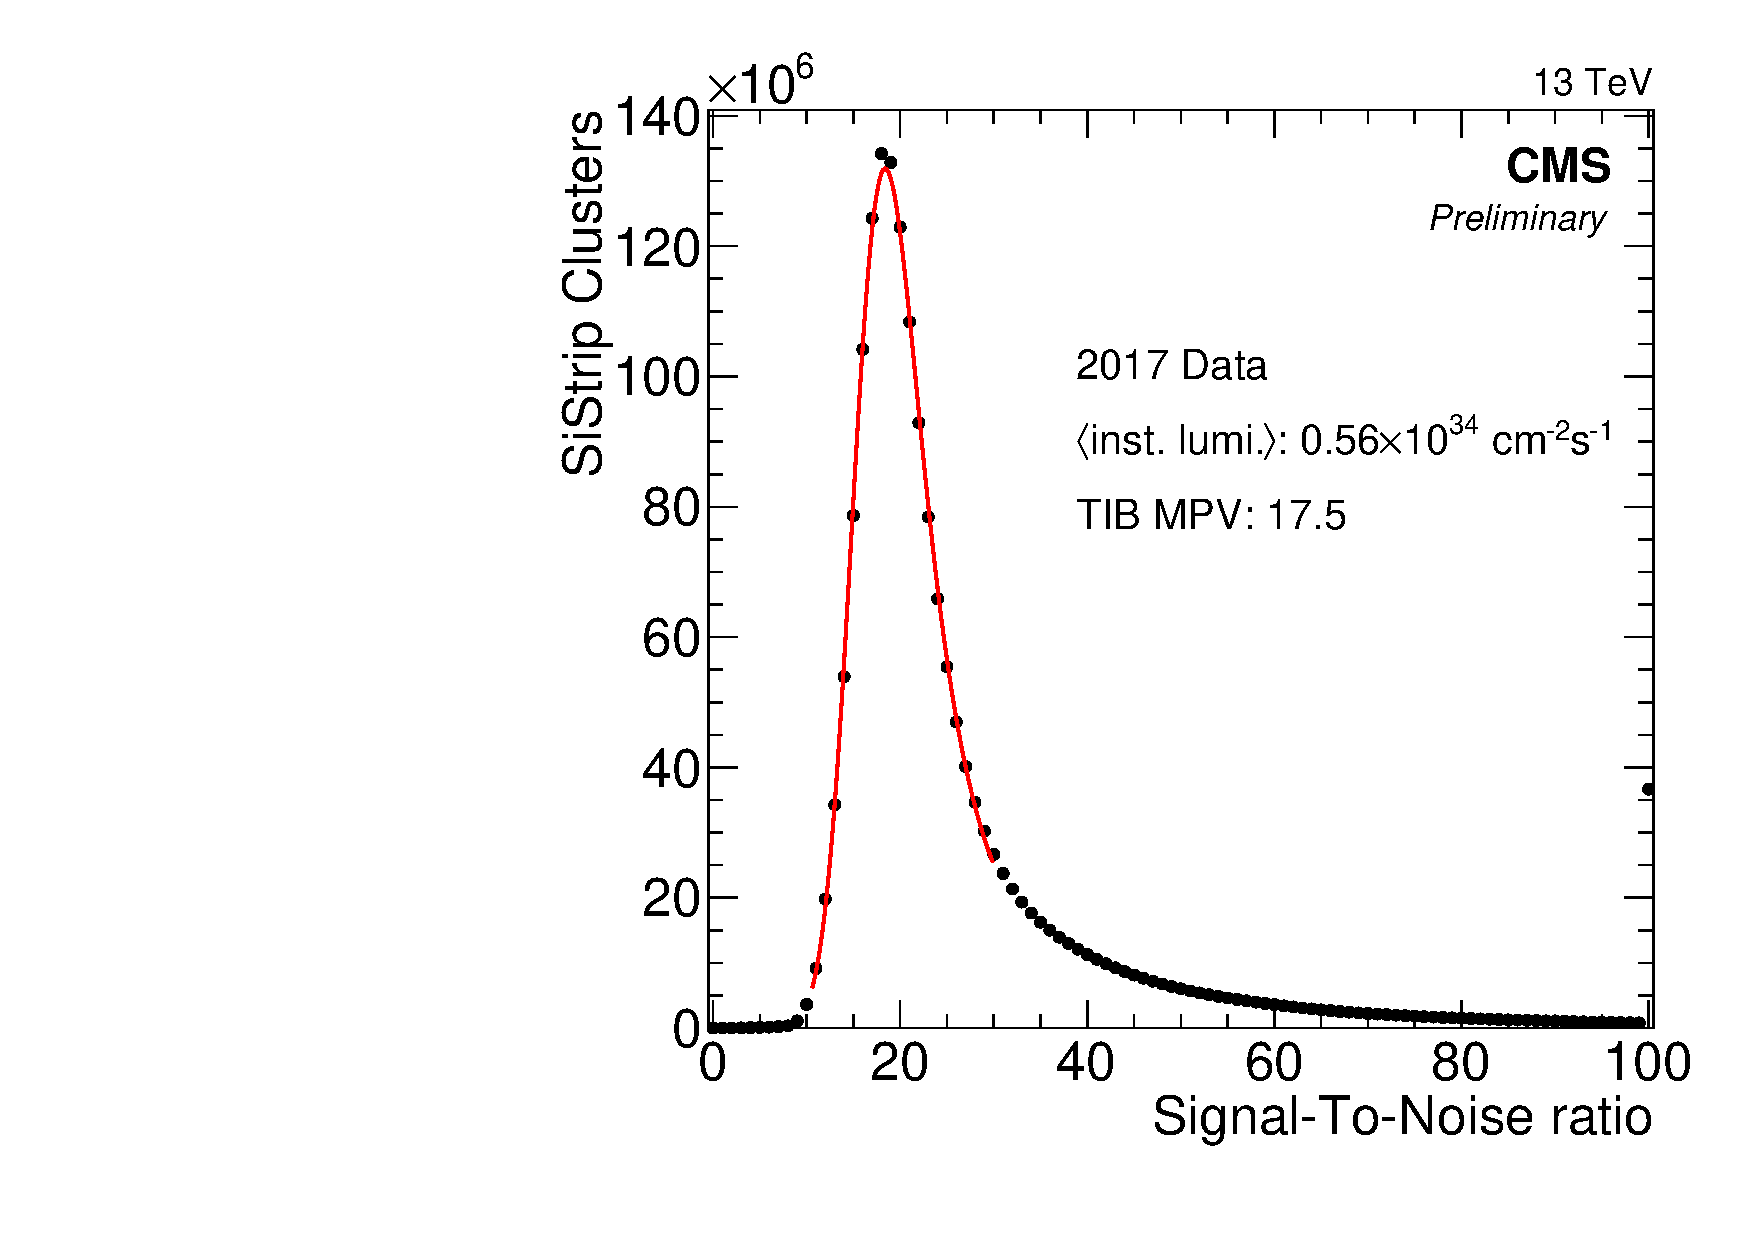
\includegraphics[height=.25\textheight]{Images/CMS/Tracker/StripTracker_SON_TIB_SOverN_run296786_2017A.pdf}}%
    \qquad
    \subfloat[Run 2 problematic channel fraction ]{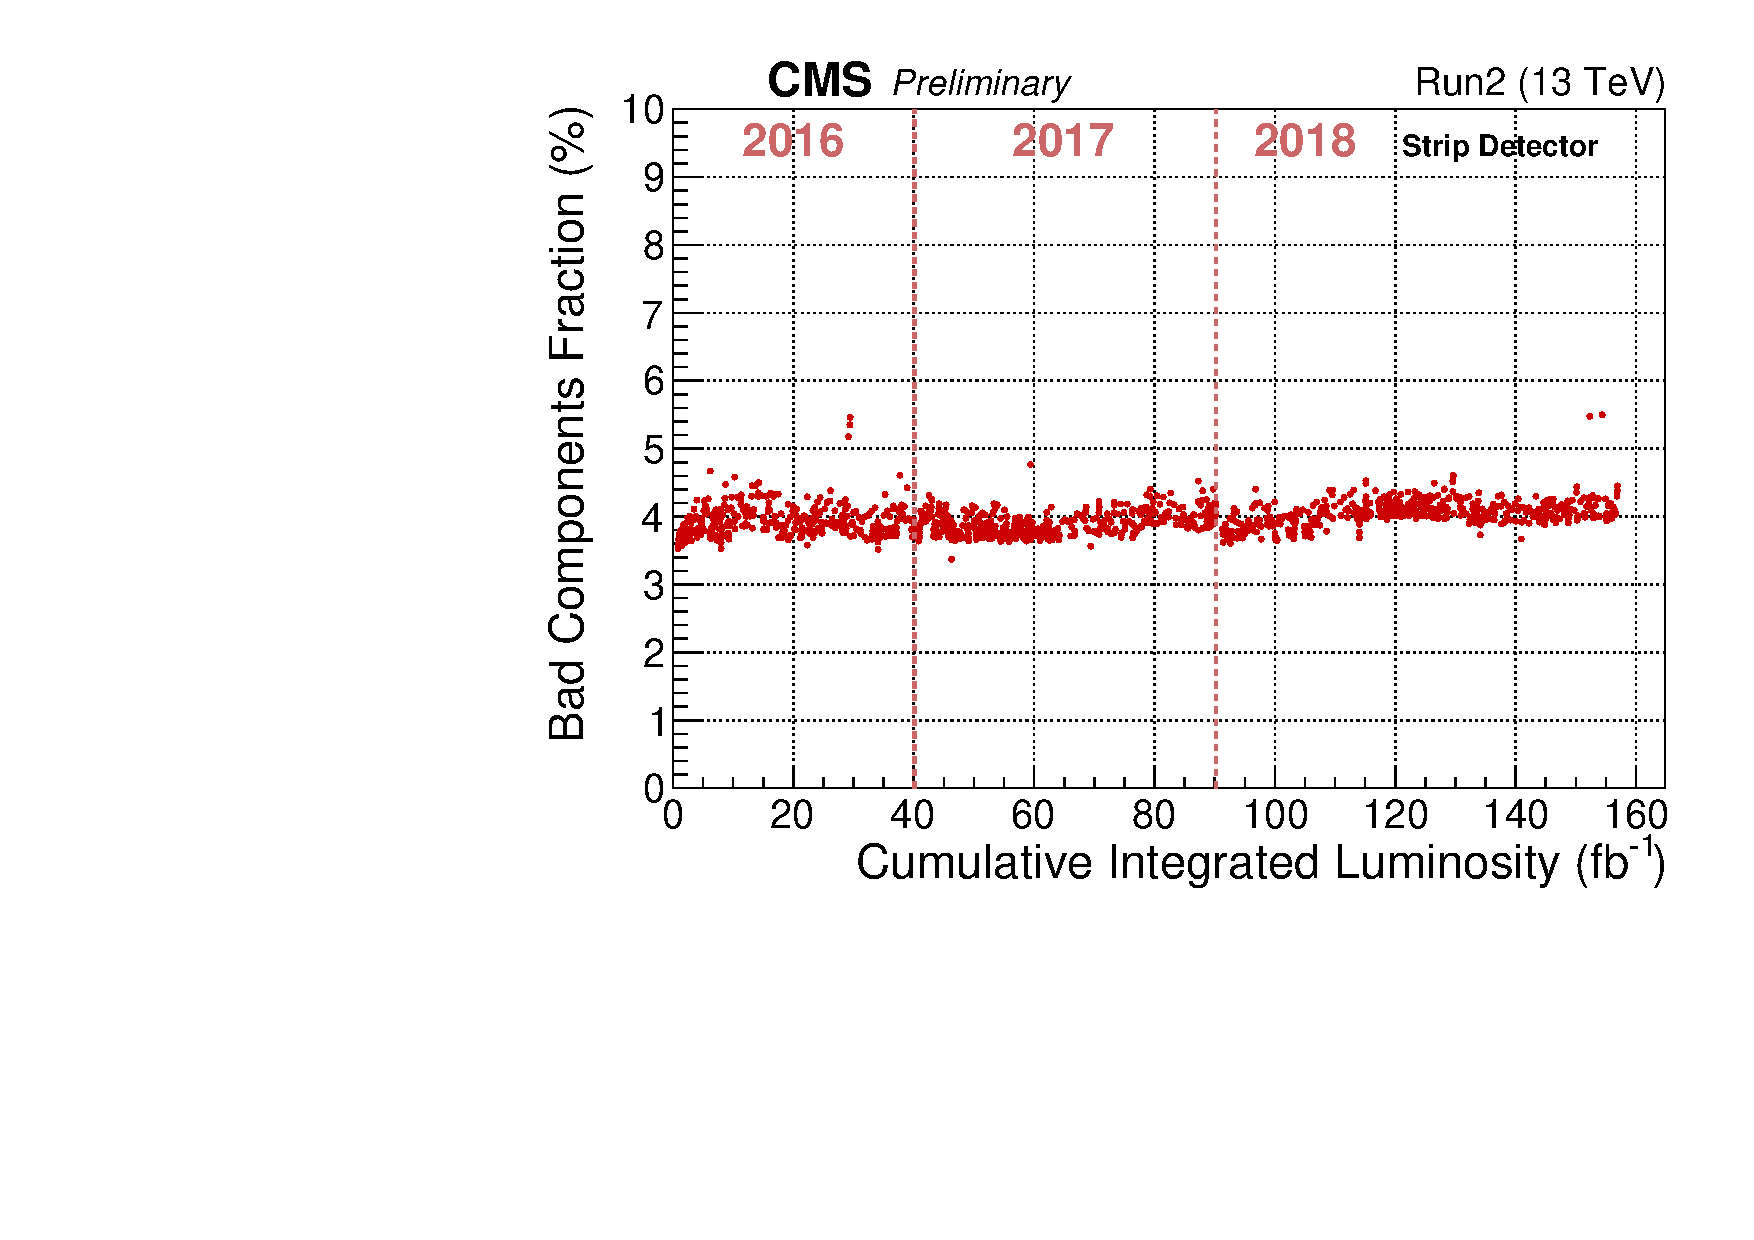
\includegraphics[height=.25\textheight]{Images/CMS/Tracker/run2_stripBadComponent_All.pdf}}%
    \caption{Run 2 strip tracker performance.} \label{fig:Run2_StripTracker}
\end{figure}  

In 2017, TIB had an excellent MPV (Most probable value) of 17.5 as a signal-to-noise ratio, indicating good signal detection in the strip tracker partition closest to the CMS interaction point. Additionally, over the course of Run 2 operations the percentage of bad components remain stable at about 4\% even after receiving the full Run 2 intergrated luminosity, highlighting the robustness of the detector. 